\documentclass[a4paper]{article}

\usepackage[czech]{babel} %https://github.com/michal-h21/biblatex-iso690
\usepackage[
   backend=biber      % if we want unicode 
  ,style=iso-numeric % or iso-numeric for numeric citation method          
  ,babel=other        % to support multiple languages in bibliography
  ,sortlocale=cs_CZ   % locale of main language, it is for sorting
  ,bibencoding=UTF8   % this is necessary only if bibliography file is in different encoding than main document
]{biblatex}

\usepackage[utf8]{inputenc}
\usepackage{fancyhdr}
\usepackage{amsmath}
\usepackage{amssymb}
\usepackage[left=2cm,right=2cm,top=2.5cm,bottom=2.5cm]{geometry}
\usepackage{graphicx}
\usepackage{pdfpages}
\usepackage{url}
\usepackage{upgreek}

\usepackage{siunitx}
\sisetup{locale = DE}  %, separate-uncertainty = true    kdybych chtel +/-

\usepackage{float}
\newfloat{graph}{htbp}{grp}
\floatname{graph}{Graf}
\newfloat{tabulka}{htbp}{tbl}
\floatname{tabulka}{Tabulka}

\renewcommand{\thefootnote}{\roman{footnote}}

\pagestyle{fancy}
\lhead{Praktikum IV - (A1) Objevování částic v detektoru ATLAS v CERN}
\rhead{Vladislav Wohlrath}
\author{Vladislav Wohlrath}

\bibliography{source}

\begin{document}

\begin{titlepage}
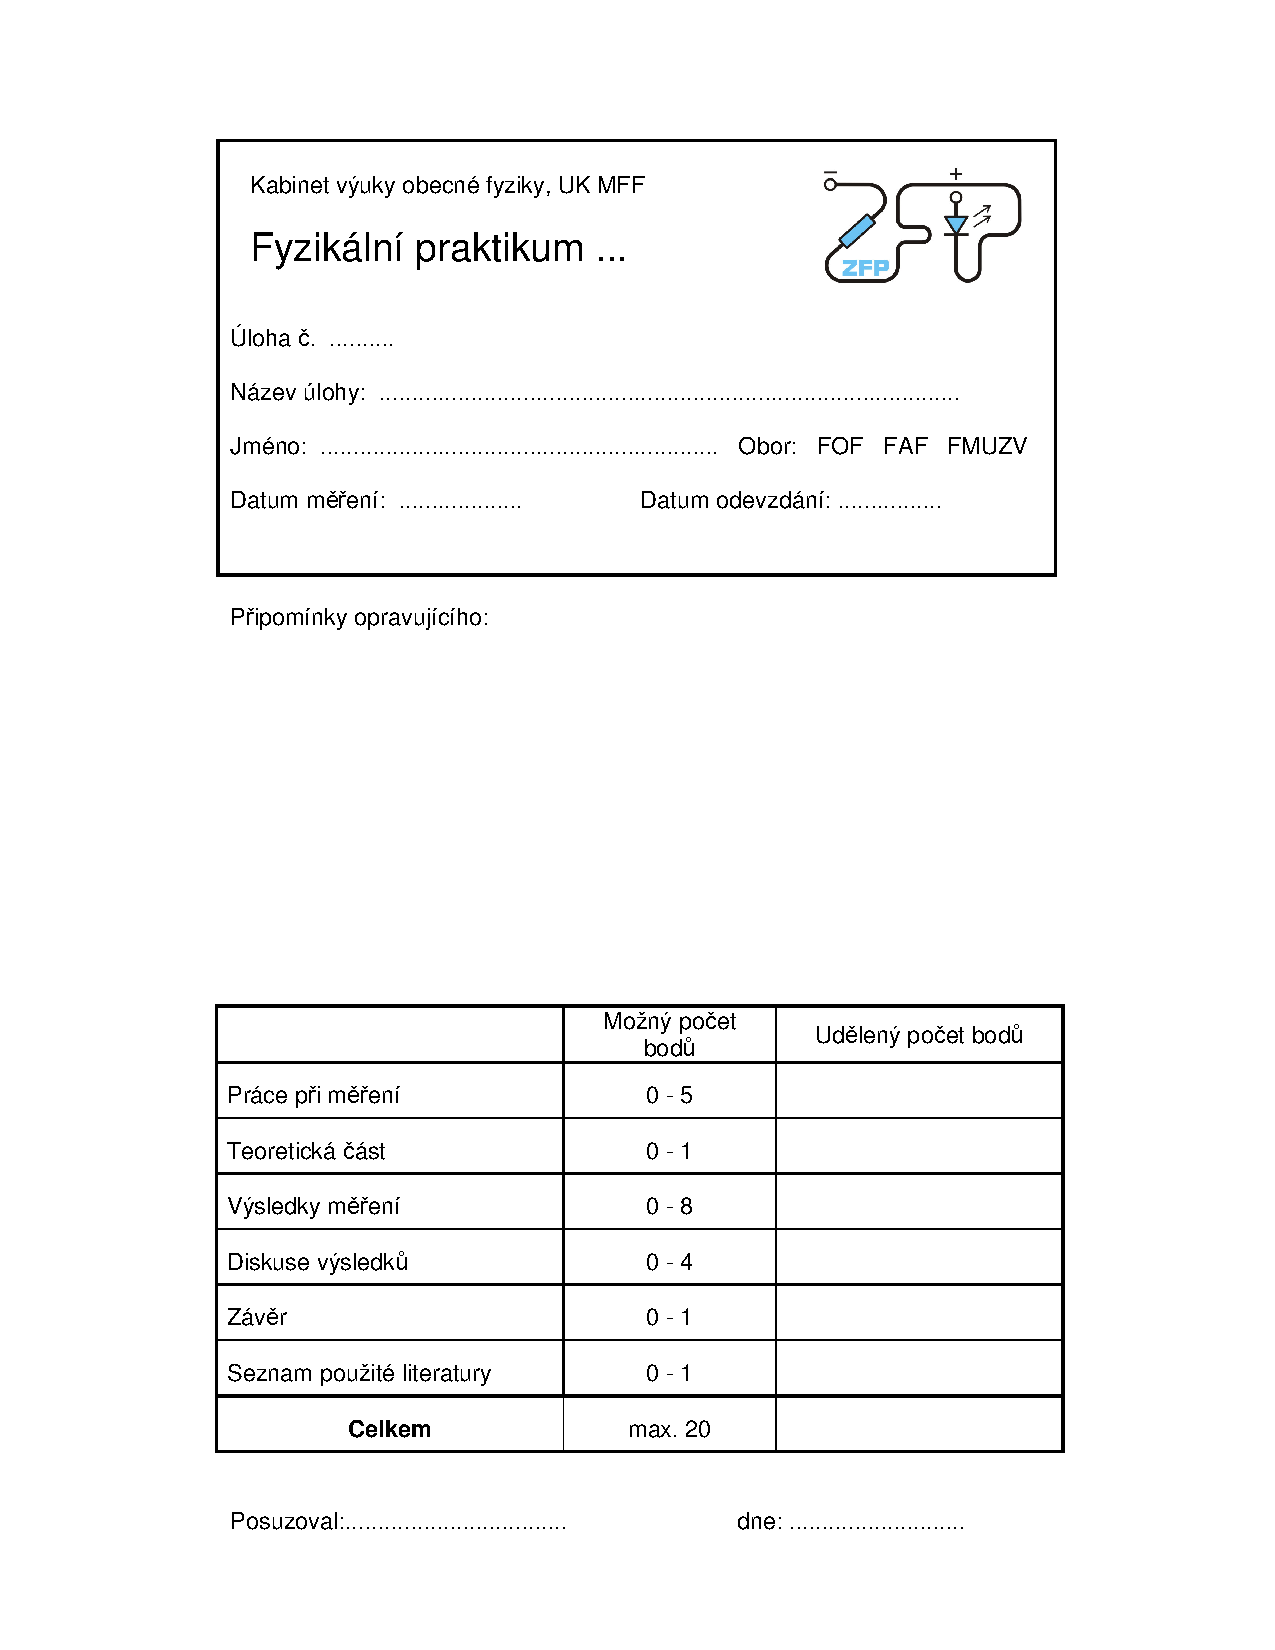
\includepdf[pages={1}]{./graficos/titlelist.pdf}
\end{titlepage}

\section*{Pracovní úkoly}
\begin{enumerate}
\item Zpracujte přibližně 50 událostí z detektoru ATLAS programem Hypatia.
\item Pomocí programu ROOT zobrazte histogram invariantních hmotností pro různě velké statistické soubory.
\item Identifikujte výrazné píky a přiřaďte je očekávaným částicím.
\item Zjistěte chybu střední hodnoty invariantní hmotnosti pro nalezené částice pro různě velké statistické soubory.
\item Vyneste zjištěné chyby do grafu jako funkci počtu událostí a srovnejte je s Poissonovým rozdělením.
\end{enumerate}

%Teoretická část
\section*{Teoretická část}

%Výsledky měření
\section*{Výsledky měření}
Zpracovali jsme 106 událostí, výsledné histogramy jsou označené klíčovým slovem \emph{mydata}, viz grafy \ref{o:m1}, \ref{o:m2}, \ref{o:m3}, \ref{o:m4}.

Soubor jsme poté rozšířili na 1370 událostí z archivu událostí zpracovaných jinými studenty. Histogramy jsou označené klíčovým slovem \emph{alldata}, viz grafy \ref{o:a1}, \ref{o:a2}, \ref{o:a3}, \ref{o:a4}.

Jasný peak okolo \SI{91}{\GeV\per $c^2$} odpovídá bosonu Z. Nasvědčuje tomu i to, že tento peak zmizí, pokud si zobrazíme pouze fotonové události.

Naopak peak okolo \SI{125}{\GeV\per $c^2$}, který je zřetelný pouze u fotonových událostí, odpovídá Higgsovu bosonu.

Ve velmi nízkých energiích pozorujeme u dileptonových událostí další peak, který podle \cite{skripta} odpovídá částicím J/$\uppsi$ a $\Upsilon$.

Další dva peaky jsou při energiích cca \SI{1000}{\GeV\per $c^2$} a \SI{1500}{\GeV\per $c^2$}, což by odpovídalo hypotetickým čísticím W', respektive g (graviton). Skutečně, do našeho soubory byly přimíchány simulované události právě s těmito částicemi.


V grafu \ref{o:com} jsou histogramy všech událostí pro různě velké statistické soubory v okolí bosonu Z.
Porovnáním parametrů fitovaných Gaussových funkcí zjišťujeme, že střední hodnota se téměř nemění, pouze se s rozšiřujícím souborem snižuje její nejistota. Se $\sigma$ je to podobné, pouze hodnota kolísá více. Do grafu \ref{o:chyby} jsme zanesli závislost nejistoty střední hodnoty na velikosti souboru.





\begin{graph}[htbp]
\centering
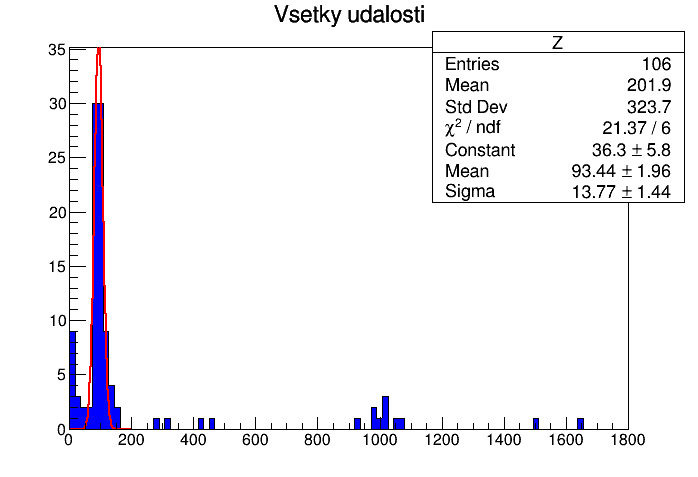
\includegraphics[width=\textwidth-2cm]{graficos/mydataz/c1_n9.png}
\caption{mydata --- všechny události}
\label{o:m1}
\end{graph}

\begin{graph}[htbp]
\centering
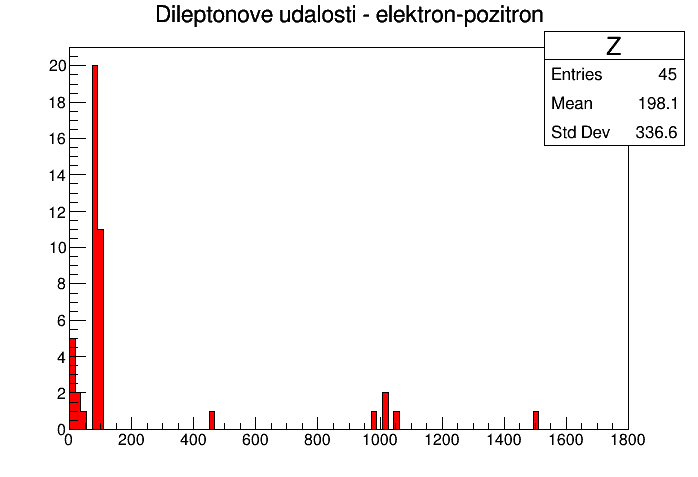
\includegraphics[width=\textwidth-2cm]{graficos/mydataz/c1_n10.png}
\caption{mydata --- elektron-pozitronové události}
\label{o:m2}
\end{graph}

\begin{graph}[htbp]
\centering
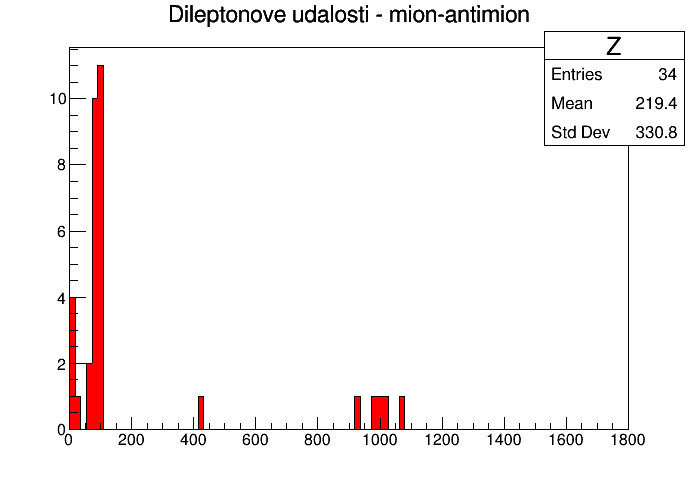
\includegraphics[width=\textwidth-2cm]{graficos/mydataz/c1_n11.png}
\caption{mydata --- mion-antimionové události}
\label{o:m3}
\end{graph}

\begin{graph}[htbp]
\centering
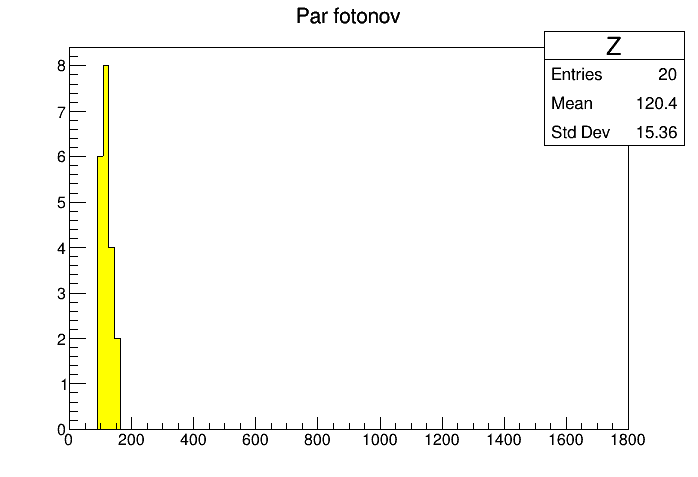
\includegraphics[width=\textwidth-2cm]{graficos/mydataz/c1_n12.png}
\caption{mydata --- dvou-fotonové události}
\label{o:m4}
\end{graph}

\begin{graph}[htbp]
\centering
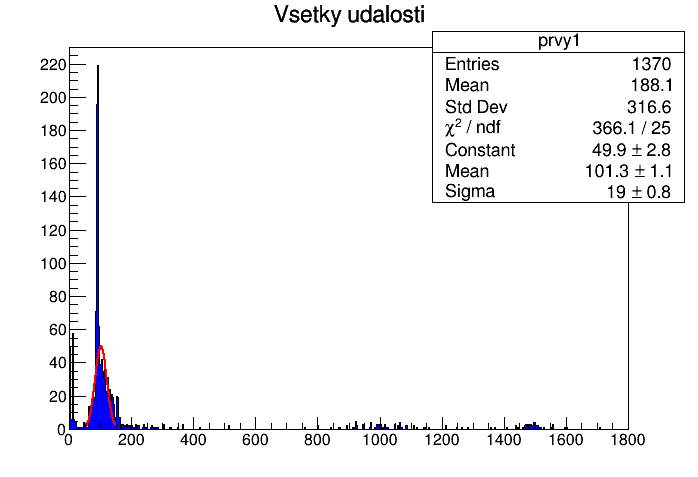
\includegraphics[width=\textwidth-2cm]{graficos/alldataz/c1.png}
\caption{alldata --- všechny události}
\label{o:a1}
\end{graph}

\begin{graph}[htbp]
\centering
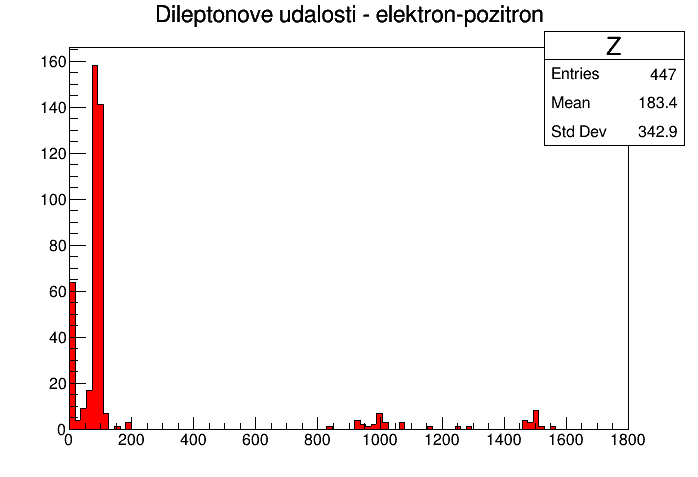
\includegraphics[width=\textwidth-2cm]{graficos/alldataz/c1_n5.png}
\caption{alldata --- elektron-pozitronové události}
\label{o:a2}
\end{graph}

\begin{graph}[htbp]
\centering
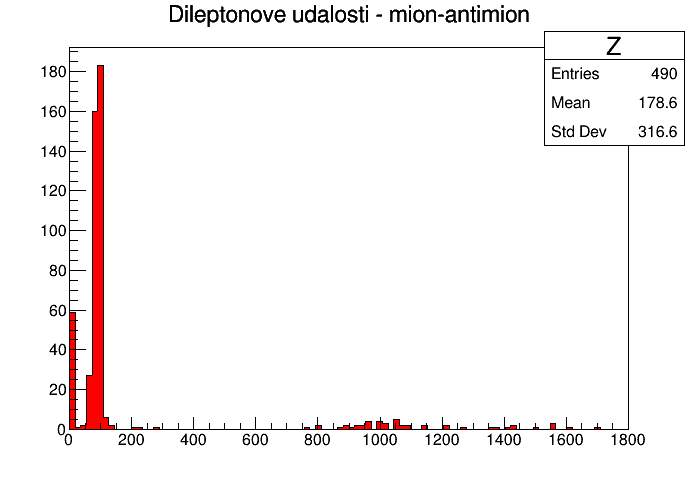
\includegraphics[width=\textwidth-2cm]{graficos/alldataz/c1_n6.png}
\caption{alldata --- mion-antimionové události}
\label{o:a3}
\end{graph}

\begin{graph}[htbp]
\centering
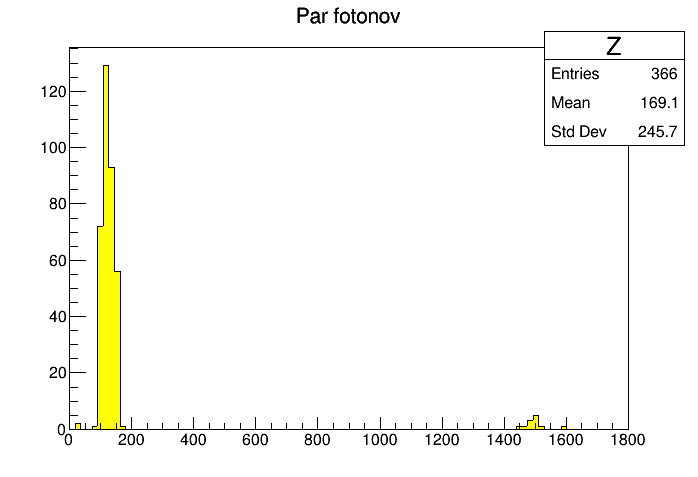
\includegraphics[width=\textwidth-2cm]{graficos/alldataz/c1_n7.png}
\caption{alldata --- dvou-fotonové události}
\label{o:a4}
\end{graph}


\begin{graph}[htbp]
\centering
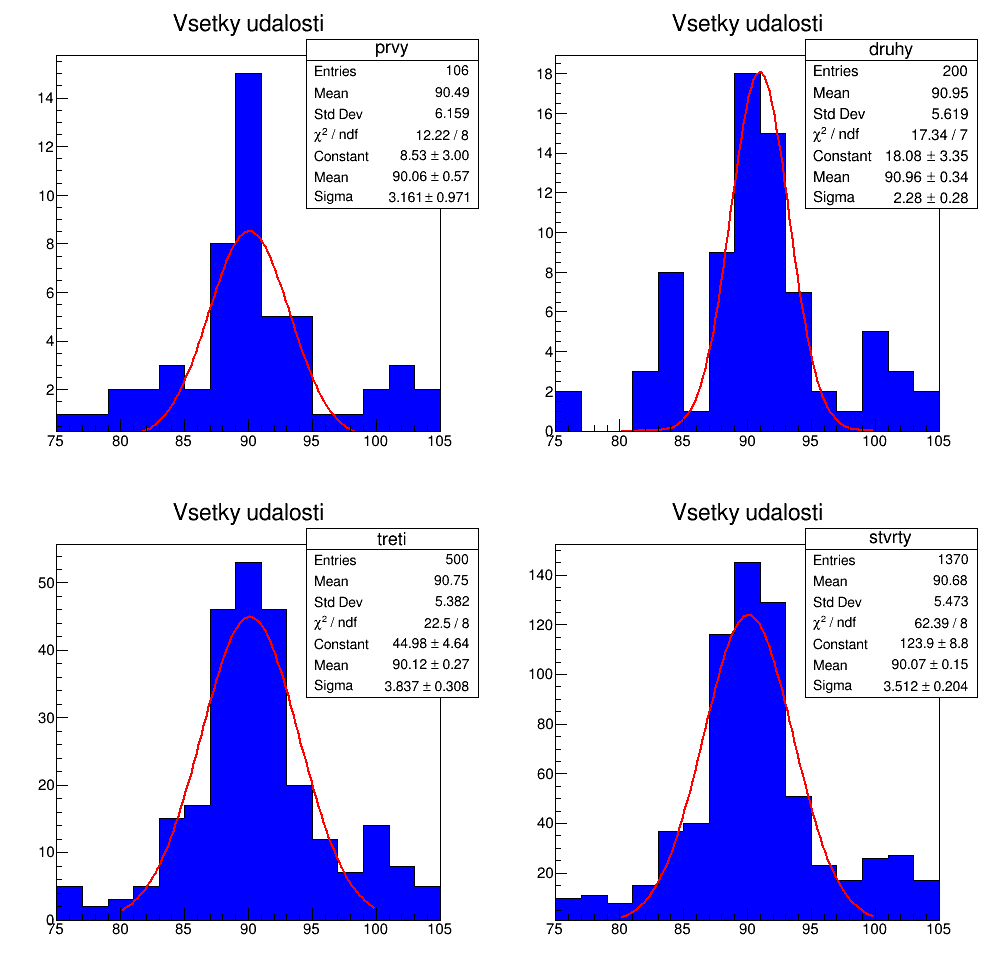
\includegraphics[width=\textwidth]{graficos/comparez/platno.png}
\caption{Porovnání histogramů pro různě velké statistické soubory.}
\label{o:com}
\end{graph}


\begin{graph}[htbp]
\centering
% GNUPLOT: LaTeX picture with Postscript
\begingroup
  \makeatletter
  \providecommand\color[2][]{%
    \GenericError{(gnuplot) \space\space\space\@spaces}{%
      Package color not loaded in conjunction with
      terminal option `colourtext'%
    }{See the gnuplot documentation for explanation.%
    }{Either use 'blacktext' in gnuplot or load the package
      color.sty in LaTeX.}%
    \renewcommand\color[2][]{}%
  }%
  \providecommand\includegraphics[2][]{%
    \GenericError{(gnuplot) \space\space\space\@spaces}{%
      Package graphicx or graphics not loaded%
    }{See the gnuplot documentation for explanation.%
    }{The gnuplot epslatex terminal needs graphicx.sty or graphics.sty.}%
    \renewcommand\includegraphics[2][]{}%
  }%
  \providecommand\rotatebox[2]{#2}%
  \@ifundefined{ifGPcolor}{%
    \newif\ifGPcolor
    \GPcolorfalse
  }{}%
  \@ifundefined{ifGPblacktext}{%
    \newif\ifGPblacktext
    \GPblacktexttrue
  }{}%
  % define a \g@addto@macro without @ in the name:
  \let\gplgaddtomacro\g@addto@macro
  % define empty templates for all commands taking text:
  \gdef\gplbacktext{}%
  \gdef\gplfronttext{}%
  \makeatother
  \ifGPblacktext
    % no textcolor at all
    \def\colorrgb#1{}%
    \def\colorgray#1{}%
  \else
    % gray or color?
    \ifGPcolor
      \def\colorrgb#1{\color[rgb]{#1}}%
      \def\colorgray#1{\color[gray]{#1}}%
      \expandafter\def\csname LTw\endcsname{\color{white}}%
      \expandafter\def\csname LTb\endcsname{\color{black}}%
      \expandafter\def\csname LTa\endcsname{\color{black}}%
      \expandafter\def\csname LT0\endcsname{\color[rgb]{1,0,0}}%
      \expandafter\def\csname LT1\endcsname{\color[rgb]{0,1,0}}%
      \expandafter\def\csname LT2\endcsname{\color[rgb]{0,0,1}}%
      \expandafter\def\csname LT3\endcsname{\color[rgb]{1,0,1}}%
      \expandafter\def\csname LT4\endcsname{\color[rgb]{0,1,1}}%
      \expandafter\def\csname LT5\endcsname{\color[rgb]{1,1,0}}%
      \expandafter\def\csname LT6\endcsname{\color[rgb]{0,0,0}}%
      \expandafter\def\csname LT7\endcsname{\color[rgb]{1,0.3,0}}%
      \expandafter\def\csname LT8\endcsname{\color[rgb]{0.5,0.5,0.5}}%
    \else
      % gray
      \def\colorrgb#1{\color{black}}%
      \def\colorgray#1{\color[gray]{#1}}%
      \expandafter\def\csname LTw\endcsname{\color{white}}%
      \expandafter\def\csname LTb\endcsname{\color{black}}%
      \expandafter\def\csname LTa\endcsname{\color{black}}%
      \expandafter\def\csname LT0\endcsname{\color{black}}%
      \expandafter\def\csname LT1\endcsname{\color{black}}%
      \expandafter\def\csname LT2\endcsname{\color{black}}%
      \expandafter\def\csname LT3\endcsname{\color{black}}%
      \expandafter\def\csname LT4\endcsname{\color{black}}%
      \expandafter\def\csname LT5\endcsname{\color{black}}%
      \expandafter\def\csname LT6\endcsname{\color{black}}%
      \expandafter\def\csname LT7\endcsname{\color{black}}%
      \expandafter\def\csname LT8\endcsname{\color{black}}%
    \fi
  \fi
  \setlength{\unitlength}{0.0500bp}%
  \begin{picture}(5668.00,4534.00)%
    \gplgaddtomacro\gplbacktext{%
      \csname LTb\endcsname%
      \put(946,704){\makebox(0,0)[r]{\strut{} 0}}%
      \csname LTb\endcsname%
      \put(946,1213){\makebox(0,0)[r]{\strut{} 0.1}}%
      \csname LTb\endcsname%
      \put(946,1723){\makebox(0,0)[r]{\strut{} 0.2}}%
      \csname LTb\endcsname%
      \put(946,2232){\makebox(0,0)[r]{\strut{} 0.3}}%
      \csname LTb\endcsname%
      \put(946,2741){\makebox(0,0)[r]{\strut{} 0.4}}%
      \csname LTb\endcsname%
      \put(946,3250){\makebox(0,0)[r]{\strut{} 0.5}}%
      \csname LTb\endcsname%
      \put(946,3760){\makebox(0,0)[r]{\strut{} 0.6}}%
      \csname LTb\endcsname%
      \put(946,4269){\makebox(0,0)[r]{\strut{} 0.7}}%
      \csname LTb\endcsname%
      \put(1078,484){\makebox(0,0){\strut{} 0}}%
      \csname LTb\endcsname%
      \put(1637,484){\makebox(0,0){\strut{} 200}}%
      \csname LTb\endcsname%
      \put(2196,484){\makebox(0,0){\strut{} 400}}%
      \csname LTb\endcsname%
      \put(2755,484){\makebox(0,0){\strut{} 600}}%
      \csname LTb\endcsname%
      \put(3314,484){\makebox(0,0){\strut{} 800}}%
      \csname LTb\endcsname%
      \put(3873,484){\makebox(0,0){\strut{} 1000}}%
      \csname LTb\endcsname%
      \put(4432,484){\makebox(0,0){\strut{} 1200}}%
      \csname LTb\endcsname%
      \put(4991,484){\makebox(0,0){\strut{} 1400}}%
      \put(176,2486){\rotatebox{-270}{\makebox(0,0){\strut{}nejistota střední hodnoty (\si{\GeV\per $c^2$})}}}%
      \put(3174,154){\makebox(0,0){\strut{}N}}%
    }%
    \gplgaddtomacro\gplfronttext{%
      \csname LTb\endcsname%
      \put(4284,4096){\makebox(0,0)[r]{\strut{}naměřená data}}%
      \csname LTb\endcsname%
      \put(4284,3876){\makebox(0,0)[r]{\strut{}$5,57/\sqrt{N}$}}%
    }%
    \gplbacktext
    \put(0,0){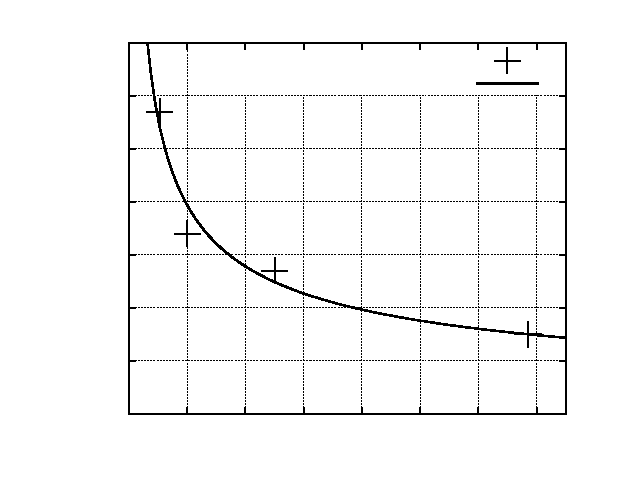
\includegraphics{chyby}}%
    \gplfronttext
  \end{picture}%
\endgroup

\caption{Závislost nejistoty určení střední hodnoty hmotnosti bosonu Z na počtu zpracovaných událostí.}
\label{o:chyby}
\end{graph}

%Diskuze výsledků
\section*{Diskuze}
Grafy jsme pozorovali v logaritmické škále na ose $y$, bohužel jsme je ale uložili v lineární škále.

Kvalitativně jsou všechny grafy mydata shodné s alldata. Pouze graviton jsme na grafu \ref{o:m4} nezaregistrovali ani jeden, což je pochopitelné vzhledem k velikosti souboru.

V grafu \ref{o:chyby} je vidět, že nejistota skutečně poměrně přesně klesá úměrně $1/\sqrt{N}$.

%Závěr
\section*{Závěr}
Zpracovali jsme 106 událostí.

Na histogramech jsme rozpoznali boson Z a Higgsův boson, dále simulované Z' a g, a pravděpodobně také J/$\uppsi$ a $\Upsilon$ viz grafy \ref{o:m1} až \ref{o:a4}.

Zobrazili jsme si histogramy pro různě velké statistické soubory. 


\printbibliography[title={Seznam použité literatury}]

\end{document}